\chapter{Multi-planar Reconstruction}
\vspace{-10mm}
\label{multiplanar}



Multi-planar Reconstruction (MPR) in medical imaging is a way of displaying three-dimensional images, captured on an imaging device. A three-dimensional study is displayed in three orthogonal slices. In each slice, there are indicated positions of the other two slices - each slice includes two lines giving the positions (See Figure \ref{fig:multiplanar}). The slices are most often parallel to basic anatomy planes\cite{ctteachingmanual}: sagittal, coronal and transverse plane.  Implementation of Multi-planar Reconstruction was requested by IKEM.

\begin{figure}
 	\caption{Multi-planar reconstruction in Dicom-Presenter.\label{fig:multiplanar}}
	\begin{center}
	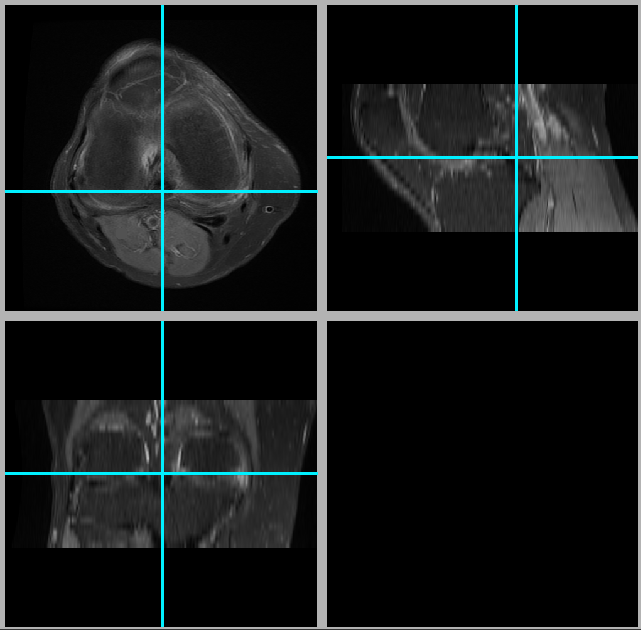
\includegraphics[width=0.75\textwidth]{Text/IMG/MultiPlanar.png}
	\end{center}
\end{figure}

\section{Designing an Object Model of Multi-planar Reconstruction}

An implementation of MPR could be divided into three parts:

\begin{itemize}
\item Handling user control. %User has to be able to freely manipulate with the three planes. Is existing
\item Image Rendering. %Is it possible to use existing classes to render three planes of a DICOM study?
\item Integration to existing object model. %The questions are, where to place the new class in the existing class hierarchy (see Section \ref{dpobjectmodel}) and how much functionality of the new class can be inherited from existing classes.
\end{itemize}

The question to discuss in all three steps is, how much of existing functionality can be used and what parts are necessary to be implemented. It is possible to implement a completely new class, which will handle user control and rendering itself. But it would lead to multiple implementations of similar tasks. The aim is to use maximum of existing functionality.

The functionality of new classes performing Multi-planar reconstruction will be similar to existing classes: Workspace and Image. Workspace class manages placement of images on the computer screen - similarly, three slices of MPR will be placed on computer screen. There is a process of obtaining proper slice from a three-dimensional image in the Image class. When using MPR, three slices will be taken in three orthogonal planes.

The similarities to Image and Workspace classes could be solved in several ways:

\begin{itemize}
\item It is possible to create a new standalone class, which will have partially similar functionality to the existing one.
\item The new functionality can be added to the existing class.
\item The existing class can be inherited by the new class.
\item An identical functionality of the class and existing class can be extracted into an abstract class, which will be inherited by both of them.
\end{itemize}

The most importance was given to the fourth option, because unlike the first option it does not add source code repetition. In addition it does not lead to creating classes with great volume of rarely used source code unlike the second option.

\section{Implementation Process of Multi-planar Reconstruction}

The class of Multi-planar Reconstruction (further MPR Workspace class), which will hold simillar function as the Workspace, was implemented as a new standalone class. The class has firmly defined layout of including images and respones to mouse events are re-defined. The MPR class owns one object of Image type. New functions for MPR rendering were added to the existing Image class.

This solution is fully functional, but it has two disadvanteges:

\begin{itemize}
\item Firsly, the MPR functions added to the Image class were constantly unused outside MPR.
\item Secondly, a relation between a Workspace and Images is different to relation between MPR Workspace and displayed Images. The MPR Workspace includes one Image object, which is responsible for rendering all three slices. More reasonable solution would be, that MPR Workspace would own three Image objects, each of them responsible for rendering one slice. This scheme corresponds to previous understandings of Image and Workspace. But moreover it would allow the three slices to by fully adjustable like an ordinary Image object (position, size, zoom, ...). 
\end{itemize}

To remove the first complaint, it will be needed to add the MPR functions to a new class and inherit the existing Image class. To avoid the second disadvantage, it will be needed to change the object design of MPR:

\begin{itemize}
\item The responsibilities of processing the user input will be shifted from the MPR Workspace class to the Image class.
%\item Then, it will be possible to allow moving and resizing the MPR Images along the Workspace easily\footnote{The Image position will be bound to the Image GUI.}.
\item The next step will be creating an abstract class describing the positions of all three slices.
\item Afterwards, three Image classes will be used for rendering the MPR. Then, the images will be fully accessible for manipulation.
\end{itemize}



